% Motivation
%

\chapter{Einleitung}

Der Einsatz von MRTs ermöglicht es Ärzten einen Einblick in das innere des menschlichen Körpers zu erlangen, ohne diesen dabei zu verletzten. Sie erhalten Bilder innerer Organe, anhand derer sich dessen Aufbau und Funktionalität beobachten lassen. Aber auch mögliche Fehlfunktionen oder Anomalien können so erfasst werden. So können auf MRT-Scans gebrochene Knochen, innere Verletzungen oder Schlaganfälle erkannt und beurteilt werden. Im Fall von Schlaganfällen kann ein MRT aufzeigen welcher Bereich des Gehirns von diesem betroffen ist, und welchen Umfang der Schaden hat.
% Wie genau?
Um den Fall eines Patienten richtig beurteilen zu können ist es unabdingbar, dass der Arzt eine möglichst umfassende Vorstellung von der Struktur des Gehirns des Patienten und vor allem von den vom Schlaganfall betroffenen Bereichen hat. Nur wenn dies der Fall ist, kann eine sinnvolle Therapie angewandt werden.
Diese Arbeit stellt die Möglichkeit vor den Umgang mit MRT-Daten anschaulicher und intuitiver zu gestalten, um somit die Arbeit von Radiologen im Bereich der Schlaganfallbehandlung zu erleichtern und die Gesundheit ihrer Patienten zu verbessern.

\begin{figure}[!htb]
	\centering
	%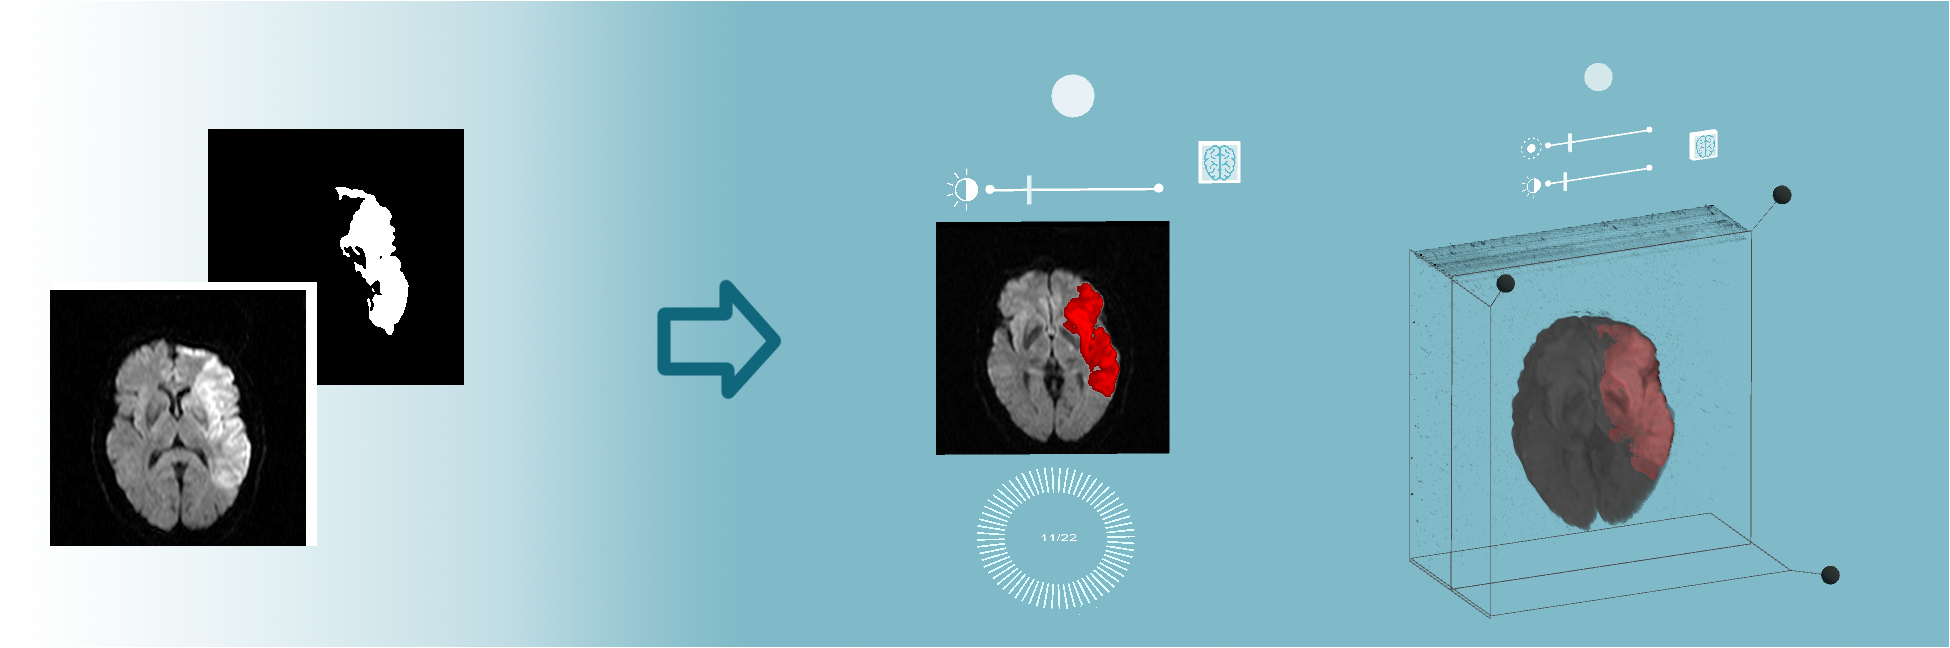
\includegraphics[width=0.3\linewidth]{images/teaser.png}
	\caption{}
	\label{img:teaser}
\end{figure}
\FloatBarrier

\section{Motivation}
\label{motivation}

Um MRT-Scans zu studieren benutzen Ärzte in der Regel speziell dafür entwickelte Software. Diese stellt das Gehirn meist aus drei verschiedenen Blickwinkeln dar, sodass es von allen Seiten zusehen ist. Entlang dieser Achsen kann der Nutzer die Ansicht durch die Schichten des Scans bewegen. Die aktuelle Position der gerade angezeigten Schicht wird in jeder der anderen Achsenansichten farbig eingezeichnet, um dem Nutzer ein möglichst umfassendes Bild des gescannten Gehirns zu vermitteln. 
Beispiele für solche Software werden im Abschnitt \ref{radiologieSoftware} näher erläutert.
%Ein Beispiel für die Oberfläche solch einer eben beschriebenen Software ist in Abbildung \ref{images/mrtSoftware} zu sehen. 
% Grundlagen?
%\todo{Bild einfügen}

Die zweidimensionale Ansicht, in der die Bilder vorliegen können allerdings eine falsche Vorstellung von der vorliegenden Situation schaffen. 
%Refrerenz?
Durch die Reduzierung um eine Dimension entsteht ein verzerrtes Bild des Gehirns. Die Darstellung der verschiedenen Achsen auf den Scans soll den Arzt bei der Orientierung unterstützen. Da das Gehirn allerdings durch mehrere Bilder dargestellt wird ist es diesem nicht möglich den Zustand auf einen Blick zu erfassen. Stattdessen müssen die Informationen aus zwei oder mehr Bildern im Kopf zusammengesetzt werden, was ein gewisses räumliches Vorstellungsvermögen voraussetzt. Dies ist ein kognitiver Aufwand, der Ärzte zusätzlich belastet, während sie sich darauf konzentrieren Anomalien in den Scans eines Patienten zu erkennen und einzuschätzen. 

Wird auf einem Scan ein Schlaganfall entdeckt, ist es durch die Abstraktion des Organs schwierig eine korrekte Vorstellung von der Größe und Lage des betroffenen Bereichs zu bekommen, da jeweils nur eine Schicht des Gehirns sichtbar ist. 
Eine dreidimensionale Ansicht des gescannten Gehirns würde einen sehr viel deutlicheren Einblick in den Zustand des Patienten liefern. Vor allem der vom Arzt gekennzeichnete betroffene Bereich wäre in 3D um einiges anschaulicher. Dies ist nicht nur für den behandelnden Arzt hilfreich. Durch die klare und eindeutigere Darstellung fällt es auch leichter den anderen die Situation zu erläutern. Dies trifft auf Patienten zu oder auch auf andere Ärzte, die der behandelnde Arzt eventuell in den Fall mit einbeziehen möchte.

Schließlich würde eine 3D-Darstellung auch das Verständnis in Lernzwecken begünstigen.
Da der betroffene Bereich in einer 3D-Darstellung auf einen Blick erfasst werden kann, eignet sie sich außerdem, um den direkten Vergleich zwischen zwei zuständen zu ziehen. So fiele es leichter beispielsweise die Größe des Bereichs vor und nach einer Therapie gegenüberzustellen, um deren Erfolgt zu demonstrieren oder zu beurteilen.
Auch Voraussagen von Therapieerfolgen könnten anschaulich demonstriert werden.

% UX  
% Software zum Vergleichen finden
Um die Anschaulichkeit und Plastizität der 3D-Darstellung voll zur Geltung zu bringen muss sie auch im dreidimensionalen Raum platziert werden. Eine volumetrische Darstellung der Daten in einer Bildschirmanwendung ist nur eine Projektion auf eine zweidimensionale Fläche. Die Darstellung wird dabei abstrahiert und der Nutzer kann nicht direkt mit dem Objekt interagieren.
Die Platzierung des 3D-Objekts in der dreidimensionalen Welt des Nutzers löst diese Barrieren auf. AR- und VR-Technologien ermöglichen sowohl die Visualisierung von dreidimensionalen virtuellen Objekten in der Umgebung des Nutzers, als auch die direkte Interaktion mit diesen. Diese gestaltet sich dabei auch deutlich intuitiver als die Bedienung eines Programms mit konventionellen Eingabemodulen, wie z.B. einer Maus. Das trifft vor allem auf tragbare AR-Brillen zu, deren Steuerung in der Regel ohne externe Steuerungsgeräte, wie Controller erfolgt. Dies ermöglicht eine verständliche und schnelle Bedienung,  was ungeübten Nutzern, wie z.B. einem Patienten oder Studenten zu Gute kommt. Die Nutzung der Anwendung wird dadurch zudem interessanter und unterhaltsamer.

Die Steuerung durch die Hände des Nutzers ist im medizinischen Bereich außerdem von besonderem Wert. So kann die Anwendung auch in sterilen Räumen oder sogar während einer Operation eingesetzt werden. In diesem Szenario kommt ein weiterer Vorteil eines tragbaren AR-Headsets zur Geltung: Durch das transparente Display kann ist es dem Nutzer möglich während der Nutzung der Anwendung seine Umgebung im Auge zu behalten. 
Eine AR-Anwendung ermöglicht es also einem Arzt während einer Operation relevante Daten abzurufen.

Durch die kabellosen, tragbaren AR-Headsets ist gleichzeitig eine höhere Mobilität gegeben, als durch einen Desktop-PC. Dadurch kann die Anwendung unabhängig von der Umgebung überall zum Einsatz kommen. 

Die Vorteile einer AR-Anwendung werden im Kapitel \ref{konzept} noch einmal erläutert.

AR-Anwendungen entwickeln sich stetig weiter und werden in der Zukunft einen immer größeren Teil des Alltags einnehmen \cite{forbes}. Diese Entwicklung wird sich voraussichtlich auch auf den medizinischen Bereich auswirken. 

Ärzte sind sich der neuen Möglichkeiten bewusst und sind daran interessiert, 
in welchen Einsatzgebieten man einen Nutzen aus diesen ziehen kann, wie \cite{holomed1} zeigen.
Eine Anwendung wie mARt eignet sich gut, um den praktischen Einsatz von AR prototypisch zu testen.

mArt bietet somit die folgenden Vorteile :

\begin{itemize}
\item 3D-Darstellung der MRT-Daten verbessert allgemeines Verständnis 
\item Direkte Interaktion mit Daten ermöglicht intuitive und ansprechende Interaktion
\item Handsteuerung und Portabilität einer AR-Anwendung ermöglichen Gebrauch im OP
\end{itemize}


\section{Zielsetzung}
% hier techniken kokretisieren

Ziel dieser Arbeit ist es, die Möglichkeiten der Darstellung von und Interaktion mit MRT-Daten in AR untersuchen. Der Fokus liegt dabei auf der Darstellung von Gehirnscans, die in der Schlaganfalldiagnose und -behandlung verwendet werden.
Hierzu soll eine prototypische Anwendung konzipiert und implementiert werden, die die eben genannten Möglichkeiten demonstriert: mARt.
Die MRT-Bilder werden innerhalb einer AR-Anwendung dreidimensional dargestellt. Außerdem soll eine möglichst intuitive Interaktion mit der Darstellung ermöglicht werden. 
Um eine nützliche Anwendung zu entwickeln, die den Anforderungen eines Einsatzes im Arbeitsfeld eines Radiologen entspricht, werden Interviews mit einem Radiologen geführt werden. Aus diesen wird dann die nötige Funktionalität der Anwendung abgeleitet. 
Die Anwendung ist nicht als einsetzbares Produkt zu verstehen sondern eher als Prototyp, der die Nützlichkeit und das Potenzial des Programms beweisen soll. Der Nutzen der Anwendung wird am Ende der Arbeit durch Nutzertests evaluiert.

\todo{Am Ende noch mal prüfen}

\section{Struktur dieser Arbeit}

Zuerst werden im  Kapitel \ref{grundlagen} theoretische Grundlagen zu Methoden und Techniken erläutert, die für das Verständnis dieser Arbeit notwendig bzw. hilfreich sind. Weiterhin werten andere Arbeiten vorgestellt,die sich mit einem ähnlichem Thema befassen oder die inhaltlich die Thematik dieser Arbeit berühren
Um die genaue Funktionalität und Umfang der zu implementierenden Anwendung festzustellen, werden in Kapitel \ref{anforderung} die Interviews mit den bereits erwähnten Radiologen ausgewertet und daraus User Stories und schließlich eine Anforderungsliste erstellt.
Anhand dieser Anforderungen wird in Kapitel \ref{konzept} ein theoretischer Entwurf der Anwendung ausgearbeitet, indem Methoden und Techniken, sowie die Benutzung des Programms diskutiert und festlegt werden.
Die Umsetzung des entwickelten Konzeptes wird schließlich in Kapitel \ref{implementierung} beschrieben. Dabei wird auch Hürden eingegangen, die im Rahmen dieser auftraten.
Das Ergebnis der Implementierung wird in Kapitel \ref{ergebnisse} dargelegt.
Die Anwendung wird anschließend getestet und mit den zuvor gestellten Anforderungen verglichen. Die Ergebnisse werden in Kapitel \ref{evaluation} beschrieben. 
In Kapitel \ref{fazit} werden die Schwerpunkte der Arbeit noch einmal zusammengefasst und mögliche Weiterentwicklungen in der Zukunft werden diskutiert. 
 